\iffalse
\let\negmedspace\undefined
\let\negthickspace\undefined
\documentclass[journal,12pt,twocolumn]{IEEEtran}
\usepackage{cite}
\usepackage{amsmath,amssymb,amsfonts,amsthm}
\usepackage{algorithmic}
\usepackage{graphicx}
\usepackage{textcomp}
\usepackage[justification=centering]{caption}
\usepackage{xcolor}
\usepackage{txfonts}
\usepackage{listings}
\usepackage{enumitem}
\usepackage{mathtools}
\usepackage{gensymb}
\usepackage{comment}
\usepackage[breaklinks=true]{hyperref}
\usepackage{tkz-euclide} 
\usepackage{listings}
\usepackage{gvv}                                        
\def\inputGnumericTable{}                                 
\usepackage[latin1]{inputenc}                                
\usepackage{color}                                            
\usepackage{array}                                            
\usepackage{longtable}                                       
\usepackage{calc}                                             
\usepackage{multirow}                                         
\usepackage{hhline}                                           
\usepackage{ifthen}                                           
\usepackage{lscape}

\newtheorem{theorem}{Theorem}[section]
\newtheorem{problem}{Problem}
\newtheorem{proposition}{Proposition}[section]
\newtheorem{lemma}{Lemma}[section]
\newtheorem{corollary}[theorem]{Corollary}
\newtheorem{example}{Example}[section]
\newtheorem{definition}[problem]{Definition}
\newcommand{\BEQA}{\begin{eqnarray}}
\newcommand{\EEQA}{\end{eqnarray}}
\newcommand{\define}{\stackrel{\triangle}{=}}
\theoremstyle{remark}
\newtheorem{rem}{Remark}
\begin{document}

\bibliographystyle{IEEEtran}
\vspace{3cm}

\title{11.9.3.6}
\author{EE23BTECH11022 - G DILIP REDDY}
\maketitle
\newpage

\bigskip

\renewcommand{\thefigure}{\theenumi}
\renewcommand{\thetable}{\theenumi}
\textbf{Question}:\\
For what values of x, the numbers $-\frac{2}{7}\,,x,-\frac{7}{2}\,$ are in G.P ?
\\\\
\textbf{Solution: }\\
\fi
\begin{table}[h]
    \centering
    \renewcommand\thetable{1}
    \begin{tabular}[12.1pt]{ |c| c| c|}
    \hline
    \textbf{Variable} & \textbf{Description} &\textbf{Value}\\ 
    \hline
    $x(0)$ & First term of the GP &$-\brak{\frac{2}{7}}$ \\
    \hline 
    $x(1)$ & Second term of the GP &$x$ \\
    \hline 
    $x(2)$ & Third term of the GP &$-\brak{\frac{7}{2}}$ \\
    \hline 
    $r$ & Common ratio of the GP & \\
    \hline
    $x(n)$ & General term & $x(0)\,r^n\,u(n)$\\
    \hline    
\end{tabular}

    \caption{Variables Used}
    \label{tab:table_11.9.3.6}
\end{table}
Let $r$ be the common ratio\\
From \tabref{tab:table_11.9.3.6}:
\begin{align}
\implies \frac{x}{\brak{-\frac{2}{7}\,}}\,&= \frac{\brak{-\frac{7}{2}\,}}{x}\,=r \\
x^2&=\brak{-\frac{2}{7}\,}\cdot\brak{-\frac{7}{2}\,}\\
x&=\pm 1\\
\implies r&=\pm \frac{7}{2}\,\\\notag
\end{align}
The signal corresponding to this is 
\begin{align}
x(n)=\brak{-\frac{2}{7}}\brak{\pm \frac{7}{2}}^n\,u(n)
\end{align}
Applying z-Transform :
\begin{align}
\implies X_1(z)&=\brak{\frac{1}{7}}\brak{\frac{4}{7z^{-1}+2}\,}
\quad \abs{z}>\frac{7}{2}\\
\implies X_2(z)&=\brak{\frac{1}{7}}\brak{\frac{4}{7z^{-1}-2}\,}
\quad \abs{z}>\frac{7}{2}
\end{align}
\begin{figure}[h]
    \renewcommand\thefigure{1}
    \centering
    \captionsetup{justification=centering}
    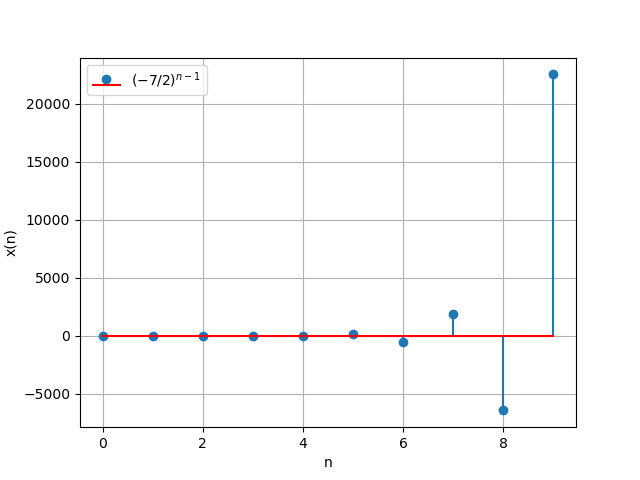
\includegraphics[width=1.1\linewidth]{ncert-maths/11/9/3/6/figs/graph1.png}
    \caption{Stem Plot of $x_1$(n)}
    \label{stemplot1}
\end{figure}
\begin{figure}[h]
    \renewcommand\thefigure{2}
    \centering
    \captionsetup{justification=centering}
    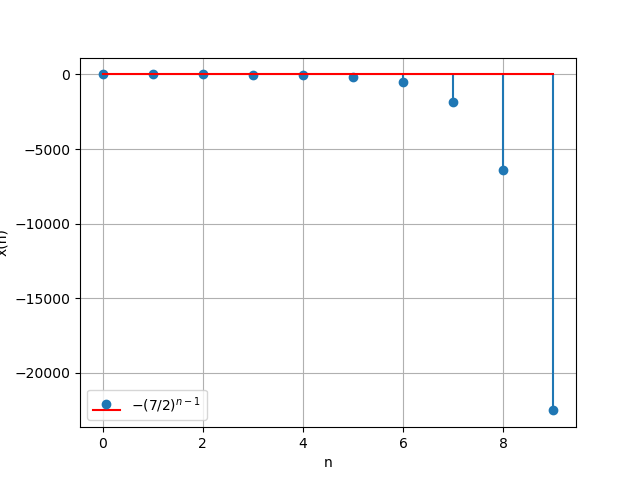
\includegraphics[width=1.1\linewidth]{ncert-maths/11/9/3/6/figs/graph2.png}
    \caption{Stem Plot of $x_2(n)$}
    \label{stemplot2}
\end{figure}
%\end{document}
